% \section{Experimental Results}\label{subsec:results:main}
% \chapter{Related Work}

\section{MITRE ATT\&CK Framework}\label{sec:related:mitre}

\section{MulVal Infrastructure Modeling}\label{sec:related:mulval}

\section{PKB}\label{sec:related:pkb}

% Before drawing any conclusions from the analysis, it should be reiterated that the results obtained rely on representative threat estimates. Refinement and feedback from an Information Assurance (IA) Officer familiar with these network architectures are needed to ensure the accuracy of the models.    

The results in this section demonstrate how comparison between architectures can be accomplished empirically using the security metrics presented in Section \ref{ch:background}. Initial parameters did not produce attack graphs for the final state model. The implication is that this architecture was 'secure' given the identified vulnerabilities, attacker origin, and target. 

To continue our analysis we conducted 'what-if' testing by introducing hypothetical vulnerabilities into the models to represent as yet unknown attacks against specific infrastructure services and devices. Testing automation allowed us to run and collect results from 20 competing models during this stage of the analysis. 


\subsubsection{Structural Metrics}\label{subsec:results:sp}
% Our findings from the structural algorithms for the three network models under test can be found in Table \ref{tab:sp_results}. The shortest path metric is a measure of the path of least resistance from an attacker's origin to the target, and can be considered a priority when identifying risk in a network. %Theoretically, it could also be used by an attacker to identify the most direct route to a target. Another consideration is that an attacker may want to determine shortest paths as part of a minimal cut set algorithm for efficiently intercepting or degrading the target’s communications. 

\begin{table}[H]
\caption{Structural Metric Results Summary}
\begin{tabular}{@{}lllll@{}}
\toprule
Structural Path Metric & Current & Transition & Final &  \\ \midrule
Shortest Path (SP) & 4 & 3 & 3 &  \\
Number of Paths (NP) & 6 & 3 & 1 &  \\
Mean Path Length (MPL) & 5.33 & 4 & 3 &  \\ \bottomrule
\end{tabular}
\label{tab:sp_results}
\end{table}

Our findings from the structural algorithms for the three network models under test can be found in Table \ref{tab:sp_results}. The shortest path metric is a measure of the path of least resistance from an attacker's origin to the target, and can be considered a priority when identifying risk in a network. %Theoretically, it could also be used by an attacker to identify the most direct route to a target. Another consideration is that an attacker may want to determine shortest paths as part of a minimal cut set algorithm for efficiently intercepting or degrading the target’s communications. 

\begin{table}[ht]
\caption{Structural Metric Results Summary}
\begin{tabular}{@{}lllll@{}}
\toprule
Structural Path Metric & Current & Transition & Final &  \\ \midrule
Shortest Path (SP) & 4 & 3 & 3 &  \\
Number of Paths (NP) & 6 & 3 & 1 &  \\
Mean Path Length (MPL) & 5.33 & 4 & 3 &  \\ \bottomrule
\end{tabular}
\label{tab:sp_results}
\end{table}

% \subsection{Node Rank}\label{subsec:results:nr}
% 
\textbf{Node Ranking (NR):  }
Figure \ref{fig:ag_all} shows the reduced attack graphs for the given models and Figure \ref{fig:nr_all} provides the corresponding Node ranks. Remember that node rank is a measure of the amount of time we expect an attacker to spend before succeeding at a given exploit, so higher values here are preferable for from a defender's point of view. We see in Figure \ref{fig:nra_fin} that  node X11 will take much longer to exploit than any other vulnerability. 
% We have shown that the elements of the fundamental matrix \(F\) take on values that represent the relative duration of time spent at each transient node in the Markov process. In the context of our security analysis, these values equate to the amount of hold time we expect an attacker to incur while trying to advance to the target. Lower node rankings indicate nodes along the attack path that are relatively easy for an attacker to clear. If a difficult to exploit vulnerability exists and its associated NR is relatively low this might be an indication that a security control point is being bypassed. Using the attack graph and associated NR analysis it is a fairly straight forward process to identify the area of interest and trace back to the origin of the bypass. Liu\cite{Liu_Singhal_Wijesekera} examines this process of forensic reconstruction of attacks using attack graphs in detail.



\begin{figure*}[ht]
\centering
\begin{adjustbox}{minipage=\linewidth,scale=.8}
\begin{subfigure}{.33\textwidth}
%\includegraphics[width=\linewidth,height=6cm]{img/1553187466086.png}
% \includegraphics[width=\linewidth,height=6cm]{content/figs/net_ags_003.png}
\includegraphics[width=\linewidth,height=6cm]{content/figs/weightedGraphs/current_007_weighEdges.png}
\caption{current}
\label{fig:ag_currt}
\end{subfigure}%
\begin{subfigure}{.33\textwidth}
%%\includegraphics[width=\linewidth,height=6cm]{img/1553187466087.png}
% \includegraphics[width=\linewidth,height=6cm]{content/figs/net_ags_002.png}
\includegraphics[width=\linewidth,height=6cm]{content/figs/weightedGraphs/transition_007_weighEdges.png}
\caption{transition}
\label{fig:ag_trans}
\end{subfigure}%
\begin{subfigure}{.2\textwidth}
%\includegraphics[width=\linewidth,height=6cm]{img/1553187466083.png}
% \includegraphics[width=\linewidth,height=5cm]{content/figs/net_ags_001.png}
\includegraphics[width=\linewidth,height=5cm]{content/figs/weightedGraphs/final_007_weighEdges.png}
\caption{final}
\label{fig:ag_fut}
\end{subfigure}%
\caption{Generated Attack Graphs}
\label{fig:ag_all}
\end{adjustbox}
\end{figure*} 


\begin{figure*}[ht]
\centering
\begin{adjustbox}{minipage=\linewidth,scale=1}
\begin{subfigure}{.33\textwidth}
\includegraphics[width=\linewidth]{img/1553187466081.png}
\caption{current}
\label{fig:nra_curr}
\end{subfigure}%
\begin{subfigure}{.33\textwidth}
\includegraphics[width=\linewidth]{img/1553187466082.png}
\caption{transition}
\label{fig:nra_trans}
\end{subfigure}%
\begin{subfigure}{.33\textwidth}
\includegraphics[width=\linewidth]{img/epl_final.png}
\caption{final}
\label{fig:nra_fin}
\end{subfigure}%
\caption{Node Rank Analysis}
\label{fig:nr_all}
\end{adjustbox}
\end{figure*} 



\textbf{Node Ranking (NR):  }

\begin{figure}[H]
\centering
% \begin{adjustbox}{minipage=\linewidth,scale=0.6}
\begin{subfigure}{.33\textwidth}
%\includegraphics[width=\linewidth,height=6cm]{img/1553187466086.png}
\includegraphics[width=\linewidth,height=6cm]{content/chapters/ch_background/sdn_analytics/2/figs/net_ags_003.png}
\caption{current}
\label{fig:ag_currt}
\end{subfigure}%
\begin{subfigure}{.33\textwidth}
%%\includegraphics[width=\linewidth,height=6cm]{img/1553187466087.png}
\includegraphics[width=\linewidth,height=6cm]{content/chapters/ch_background/sdn_analytics/2/figs/net_ags_002.png}
\caption{transition}
\label{fig:ag_trans}
\end{subfigure}%
\begin{subfigure}{.2\textwidth}
%\includegraphics[width=\linewidth,height=6cm]{img/1553187466083.png}
\includegraphics[width=\linewidth,height=5cm]{content/chapters/ch_background/sdn_analytics/2/figs/net_ags_001.png}
\caption{final}
\label{fig:ag_fut}
\end{subfigure}%
\caption{Generated Attack Graphs}
% \end{adjustbox}
\end{figure} 


\begin{figure}[H]
\centering
% \begin{adjustbox}{minipage=\linewidth,scale=0.6}
\begin{subfigure}{.33\textwidth}
\includegraphics[width=\linewidth]{content/chapters/ch_background/sdn_analytics/2/figs/weightedGraphs/current_007_weighEdges.png}
\caption{current}
\label{fig:nra_curr}
\end{subfigure}%
\begin{subfigure}{.33\textwidth}
\includegraphics[width=\linewidth]{content/chapters/ch_background/sdn_analytics/2/figs/weightedGraphs/transition_007_weighEdges.png}
\caption{transition}
\label{fig:nra_trans}
\end{subfigure}%
\begin{subfigure}{.33\textwidth}
\includegraphics[width=\linewidth]{content/chapters/ch_background/sdn_analytics/2/figs/weightedGraphs/final_007_weighEdges.png}
\caption{transition}
\label{fig:nra_fin}
\end{subfigure}%
\caption{Node Rank Analysis}
% \end{adjustbox}
\end{figure} 

\subsubsection{Expected Path Length}\label{subsec:results:epl}
% 
\textbf{Expected Path Length (EPL):  }

% We define EPL as the expected number of time steps required for an attacker to advance from the initial state to the attack goal, and its calculation follows as a direct consequence of deriving the NR metric. That is, if the NR metric expresses the total expected time that a process starting in initial state $s_i$ will occur in transient state \(s_j\) before ultimately being absorbed, then the NR sum over all transient states for \(s_i\) will predict the total time spent in the process before absorption. To take the sum of the values in the rows of the fundamental matrix we multiply by a column of 1’s, t = N1, and the entry \(t_i\) contains the EPL value for initial state \(s_i\). 
EPL describes how long we can expect an attacker to be in our network before the target is successfully compromised. Table \ref{tab:epl_result} shows the EPL values for each model along with the path length histogram of the simulations that were run. This histogram counts how many times the simulation reached the target in exactly Path Length steps. We can infer that the higher the EPL value, the longer an attacker will attempt to advance to the target, and the more chance we have to observe and act in response [1]. The long tail on the final state histogram indicates that, in several simulations, the observed path length nearly tripled that of the other two models. We notice that, despite having significantly more available attack paths (NP(current)=6 vs NP(SDN)=3) the expected path length of the current model is actually higher than that of the SDN model. Likewise, although the SDN models  both have Shortest Path scores = 3, we have shown the resiliency of these networks to be unequal.  In doing so we demonstrate the additional insight provided by incorporating vulnerability awareness into our threat modelling and planning tools.

% \begin{figure*}[ht]
\begin{table*}[ht]
\caption{Expected Path Length Results}
\resizebox{\textwidth}{!}{%
\begin{tabular}{@{}llll@{}}
\toprule
Current & Transition & Final &  \\ \midrule
Expected Length: 9.398 & Expected Length: 8.0875 & Expected Length: 11.1405 &  \\ \bottomrule
\raisebox{-\totalheight}{\includegraphics[width=0.3\textwidth, height=60mm]{img/pathlength_curr.png}}
      & 
\raisebox{-\totalheight}{\includegraphics[width=0.3\textwidth, height=60mm]{img/pathlength_trans.png}}
&
\raisebox{-\totalheight}{\includegraphics[width=0.3\textwidth, height=60mm]{img/pathlength_final.png}}
\\
\end{tabular}
}
\label{tab:epl_result}
\end{table*}

% \end{figure*}

 


\textbf{Expected Path Length (EPL):  }

% We define EPL as the expected number of time steps required for an attacker to advance from the initial state to the attack goal, and its calculation follows as a direct consequence of deriving the NR metric. That is, if the NR metric expresses the total expected time that a process starting in initial state $s_i$ will occur in transient state \(s_j\) before ultimately being absorbed, then the NR sum over all transient states for \(s_i\) will predict the total time spent in the process before absorption. To take the sum of the values in the rows of the fundamental matrix we multiply by a column of 1’s, t = N1, and the entry \(t_i\) contains the EPL value for initial state \(s_i\). 
EPL describes how long we can expect an attacker to be in our network before the target is successfully compromised. Table \ref{tab:epl_result} shows the EPL values for each model along with the path length histogram of the simulations that were run. This histogram counts how many times the simulation reached the target in exactly Path Length steps. We can infer that the higher the EPL value, the longer an attacker will attempt to advance to the target, and the more chance we have to observe and act in response [1]. The long tail on the final state histogram indicates that, in several simulations, the observed path length nearly tripled that of the other two models. We notice that, despite having significantly more available attack paths (NP(current)=6 vs NP(SDN)=3) the expected path length of the current model is actually higher than that of the SDN model. Likewise, although the SDN models  both have Shortest Path scores = 3, we have shown the resiliency of these networks to be unequal.  In doing so we demonstrate the additional insight provided by incorporating vulnerability awareness into our threat modelling and planning tools.

\begin{table}[H]
\caption{Expected Path Length Results}
\begin{tabular}{@{}llll@{}}
\toprule
Current & Transition & Final &  \\ \midrule
Expected Length: 9.398 & Expected Length: 8.0875 & Expected Length: 11.1405 &  \\ \bottomrule
\raisebox{-\totalheight}{\includegraphics[width=0.3\textwidth, height=60mm]{resource/img/ch_casestudies/att/pathlength_curr.png}}
      & 
\raisebox{-\totalheight}{\includegraphics[width=0.3\textwidth, height=60mm]{resource/img/ch_casestudies/att/pathlength_trans.png}}
&
\raisebox{-\totalheight}{\includegraphics[width=0.3\textwidth, height=60mm]{resource/img/ch_casestudies/att/pathlength_final.png}}
\\
\end{tabular}
\label{tab:epl_result}
\end{table}


 

\subsubsection{Probabilistic Path}\label{subsec:results:pp}
% 
\(
\textbf{Probabilistic Path (PP):} 
\)
% The PP metric is another interesting property derived from our Markov transition matrix. Taking the product of the fundamental matrix F and the matrix of absorbing probabilities \(R\) results in a matrix, \(B = FR\), whose \(B(i,j) \) entries yield the probability of being absorbed by state \(s_j\) given we started at initial state \(s_i\).  


\begin{figure}[H]
\centering
\includegraphics[width=100mm]{img/ag_extra_target.png}
\caption{Transition diagram with additional absorbing states New\_Target}
\label{fig:ag_pp}
\end{figure}


In the current scenario calculating this PP metric results in a column of 1’s since we only define a single ‘Target’ node in each of our models with 100\% chance of absorption from any transient node by definition.   

However it is easy to imagine a case where multiple targets are specified in the model. For example, we have added a second absorbing state, ‘New\_Target’ to the transition diagram from Figure \ref{fig:ag_2}. This could represent a hot failover clone of the existing Target or it could be a completely separate system with unique vulnerabilities. In either case we can make a grounded prediction on which state will absorb the attacker with the highest likelihood and prepare accordingly. 




\(
\textbf{Probabilistic Path (PP):} 
\)
% The PP metric is another interesting property derived from our Markov transition matrix. Taking the product of the fundamental matrix F and the matrix of absorbing probabilities \(R\) results in a matrix, \(B = FR\), whose \(B(i,j) \) entries yield the probability of being absorbed by state \(s_j\) given we started at initial state \(s_i\).  


\begin{figure}[H]
\centering
\includegraphics[width=100mm]{resource/img/ch_casestudies/att/ag_extra_target.png}
\caption{Transition diagram with additional absorbing states New\_Target}
\label{fig:ag_pp}
\end{figure}


In the current scenario calculating this PP metric results in a column of 1’s since we only define a single ‘Target’ node in each of our models with 100\% chance of absorption from any transient node by definition.   

However it is easy to imagine a case where multiple targets are specified in the model. For example, we have added a second absorbing state, ‘New\_Target’ to the transition diagram from Figure \ref{fig:ag_2}. This could represent a hot failover clone of the existing Target or it could be a completely separate system with unique vulnerabilities. In either case we can make a grounded prediction on which state will absorb the attacker with the highest likelihood and prepare accordingly. 



 



